\documentclass{article}
\usepackage{graphicx}
\usepackage[a4paper, hmargin = 2.5cm, vmargin = 2.5cm]{geometry}
\usepackage[english]{babel}

\title{Datenbankprojekt : Reisebüro/Travel agency}
\author{Oliver Baltisberger, Rachid Flueckiger, Christian Pernet}
\date{\today}

\begin{document}
	\maketitle
	
	\section*{Project description}
	Our project aims to implement a (very) simple customer relationship management database for a travel agency. 
	Several travel agencies employ collaborators. These employees sell trips to customers. 
	In our example, the trips are organized trips. They also have a begin date, a duration, a price and a category. 
	The category can be e.g. cruse, road trip, safari, ...
	
	\section*{Queries examples}
	\begin{enumerate}
		\item make a list of all employees.
		\item make a list of all employees working for a particuliar agency.
		\item count the number of trips sold by an employee.
		\item which employee has sold the highest number of trips.
		\item sum the sales made by an employee
		\item make a list of the clients.
		\item determine the preferred paiement method of the clients.
		\item determine the preferred contact method of the clients.
		\item make a list of the trips.
		\item make a list of the trips for a particuliar category.
		\item make a list of the clients who have reserved a trip.
		\item for each category, list all the reservation made by clients.
		\item determine for a sale, if the paiement is complete.
	\end{enumerate}
	
	\vspace{2 cm}
	On the next page, you find the ER-Diagram of this project. 
	
	
	\newpage
	
	\section*{ER-Diagram}
	\begin{figure}[htbp]
		\centering
			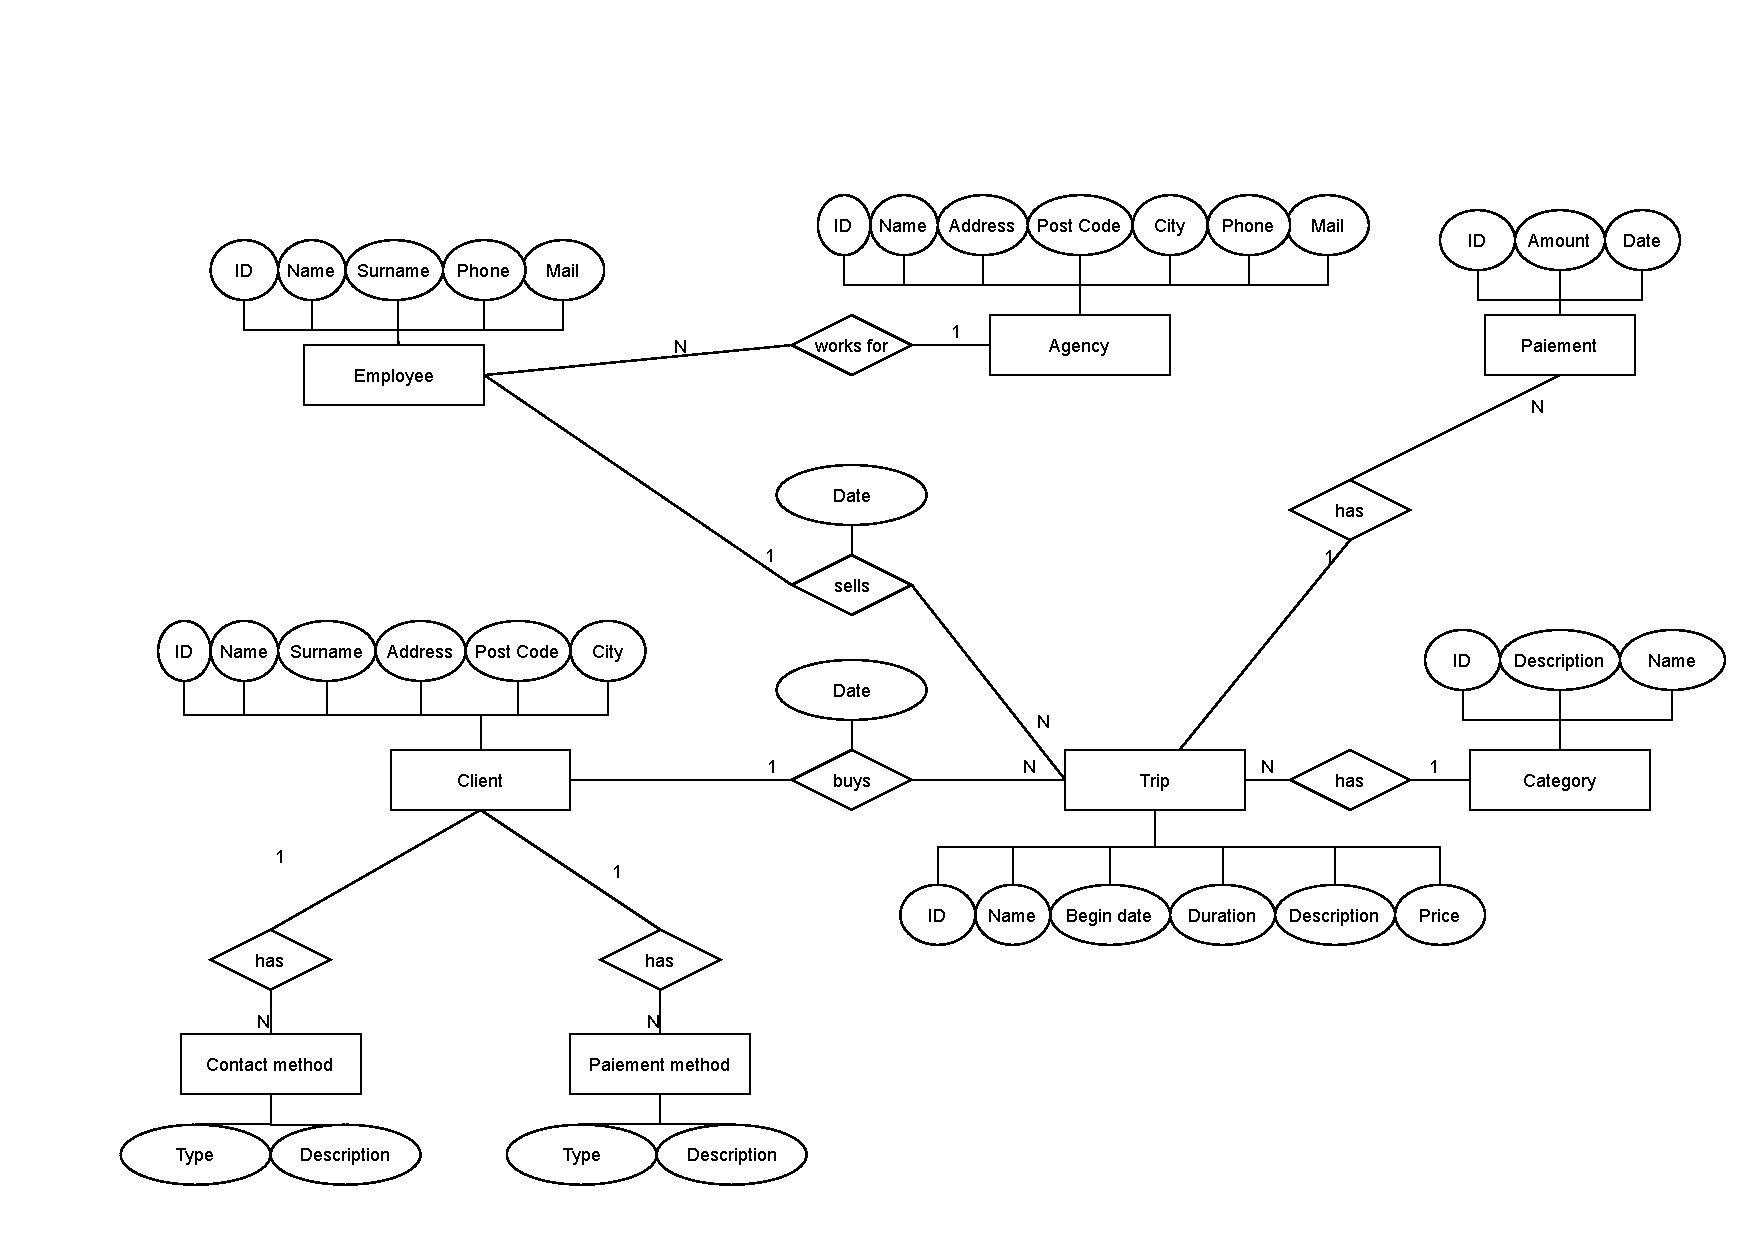
\includegraphics[width=1.00\textwidth]{../model.pdf}
		\label{ER-Model}
		\caption{Travel agency ER-Model}
	\end{figure}
	

\end{document}